\documentclass[tikz,border=12pt]{standalone}
\usepackage{tikz}
\usepackage{xcolor}

\definecolor{bluebell}{rgb}{0.25, 0.35, 0.89}
\definecolor{iris}{rgb}{0.25, 0.35, 0.89}

%% Fonte grande absoluta para os rótulos
\newcommand{\FL}{\fontsize{16}{20}\selectfont\bfseries}

\begin{document}

%% Figura 1 — Teorema de Tales (diagrama)
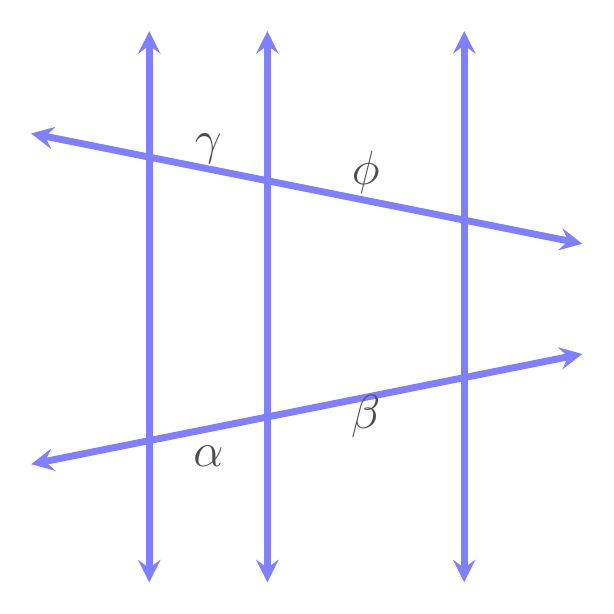
\begin{tikzpicture}
\tikzstyle{texto}=[draw=none,fill=none,black!70!white,font=\FL]
\tikzstyle{line}=[blue!50!white,line width=2.5pt]

\draw[line,stealth-stealth] (0,0) -- (7,1.4);
\draw[line,stealth-stealth] (0,4.2) -- (7,2.8);
\draw[line,stealth-stealth] (1.5,-1.5) -- (1.5,5.5);
\draw[line,stealth-stealth] (3,-1.5) -- (3,5.5);
\draw[line,stealth-stealth] (5.5,-1.5) -- (5.5,5.5);

\node[texto] at (2.25,0.1)  {$\alpha$};
\node[texto] at (4.25,0.6)  {$\beta$};

\node[texto] at (2.25,4.0)  {$\gamma$};
\node[texto] at (4.25,3.7)  {$\phi$};
\end{tikzpicture}

%% Figura 2 — Teorema de Tales (exemplo com valores)
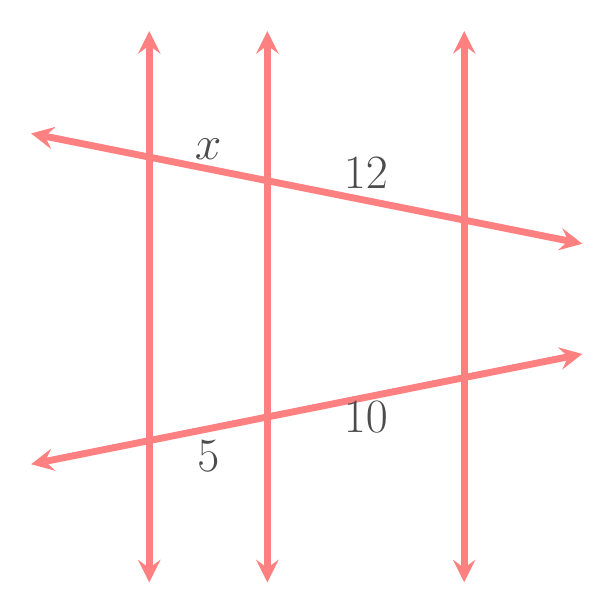
\begin{tikzpicture}
\tikzstyle{texto}=[draw=none,fill=none,black!70!white,font=\FL]
\tikzstyle{line}=[red!50!white,line width=2.5pt]

\draw[line,stealth-stealth] (0,0) -- (7,1.4);
\draw[line,stealth-stealth] (0,4.2) -- (7,2.8);
\draw[line,stealth-stealth] (1.5,-1.5) -- (1.5,5.5);
\draw[line,stealth-stealth] (3,-1.5) -- (3,5.5);
\draw[line,stealth-stealth] (5.5,-1.5) -- (5.5,5.5);

\node[texto] at (2.25,0.1)  {$5$};
\node[texto] at (4.25,0.6)  {$10$};

\node[texto] at (2.25,4.0)  {$x$};
\node[texto] at (4.25,3.7)  {$12$};
\end{tikzpicture}

%% Figura 3 — Triângulos Semelhantes (diagrama genérico)
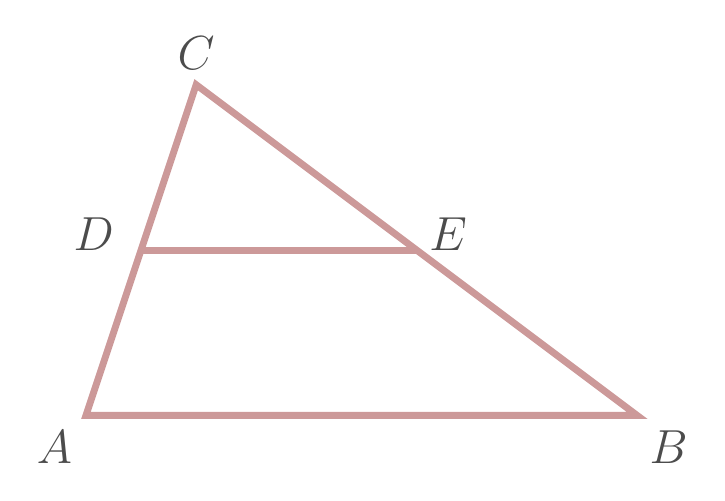
\begin{tikzpicture}
\tikzstyle{texto}=[draw=none,fill=none,black!70!white,font=\FL]
\tikzstyle{line}=[pink!80!black,line width=2.5pt]

\draw[line] (0,0) -- (7,0) -- (1.4,4.2) -- cycle;
\draw[line] (0.7,2.1) -- (4.2,2.1);

\node[texto] at (-0.4,-0.4) {$A$};
\node[texto] at (7.4,-0.4) {$B$};
\node[texto] at (1.4,4.6)  {$C$};
\node[texto] at (0.1,2.3)  {$D$};
\node[texto] at (4.6,2.3)  {$E$};
\end{tikzpicture}

%% Figura 4 — Triângulos Semelhantes (exemplo 1: x=4)
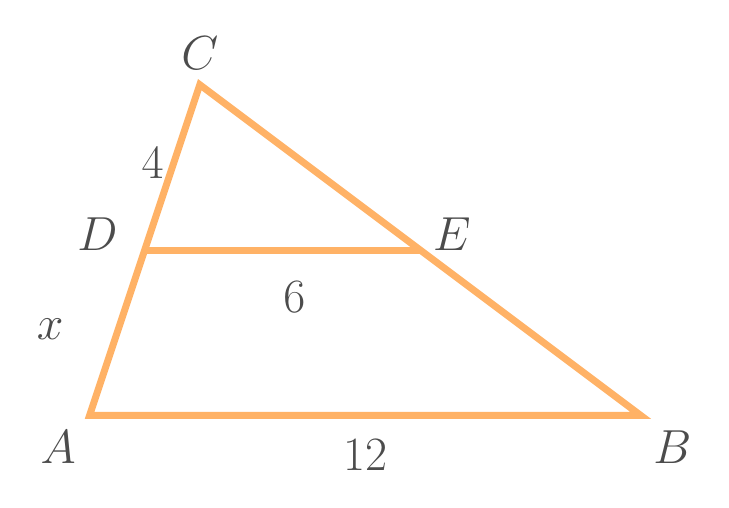
\begin{tikzpicture}
\tikzstyle{texto}=[draw=none,fill=none,black!70!white,font=\FL]
\tikzstyle{line}=[orange!60!white,line width=2.5pt]

\draw[line] (0,0) -- (7,0) -- (1.4,4.2) -- cycle;
\draw[line] (0.7,2.1) -- (4.2,2.1);

\node[texto] at (3.5,-0.5) {$12$};
\node[texto] at (2.6,1.5)  {$6$};
\node[texto] at (0.8,3.2)  {$4$};
\node[texto] at (-0.5,1.1) {$x$};

\node[texto] at (-0.4,-0.4) {$A$};
\node[texto] at (7.4,-0.4) {$B$};
\node[texto] at (1.4,4.6)  {$C$};
\node[texto] at (0.1,2.3)  {$D$};
\node[texto] at (4.6,2.3)  {$E$};
\end{tikzpicture}

%% Figura 5 — Triângulos Semelhantes (exemplo 2: x=12)
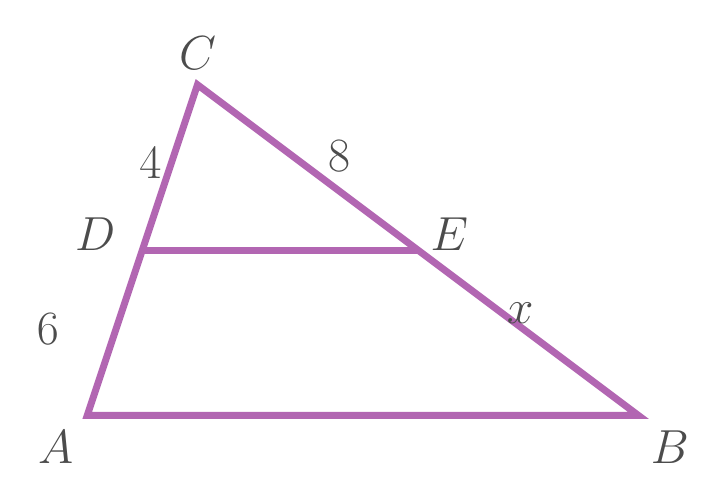
\begin{tikzpicture}
\tikzstyle{texto}=[draw=none,fill=none,black!70!white,font=\FL]
\tikzstyle{line}=[violet!60!white,line width=2.5pt]

\draw[line] (0,0) -- (7,0) -- (1.4,4.2) -- cycle;
\draw[line] (0.7,2.1) -- (4.2,2.1);

\node[texto] at (5.5,1.3)  {$x$};
\node[texto] at (3.2,3.3)  {$8$};
\node[texto] at (0.8,3.2)  {$4$};
\node[texto] at (-0.5,1.1) {$6$};

\node[texto] at (-0.4,-0.4) {$A$};
\node[texto] at (7.4,-0.4) {$B$};
\node[texto] at (1.4,4.6)  {$C$};
\node[texto] at (0.1,2.3)  {$D$};
\node[texto] at (4.6,2.3)  {$E$};
\end{tikzpicture}

\end{document}
